\documentclass{article}
\usepackage{../tex/mysty}
\usepackage[final]{pdfpages}
\begin{document}


\maketitlepage{U.S. Food and Drug Administration: Regulatory
  Report}{Sanjay Challa}

\setcounter{tocdepth}{3}
\tableofcontents
\newpage

\section*{Executive summary}
\label{sec:exec-summary}

\section{Regulation Overview}
\label{sec:test-administration}

\section{Device Classification}
\label{sec:protocols}
B. Device Classification Wt =20\% Points
a. Panels
b. 7-digit classification
c. 3-alpha code
d. Documentation on how search was conducted
e. If not regulated, state compelling argument
f. What other regulations may apply?

A search in the PRODUCT CODE CLASSIFICATION DATABASE using the
keywords: "tomography" and "ophthalmic", is done. There are few entrys
that partially describes our device. Optical coherence tomography,
product code OBO, regulation number 886.1570, describes an
ophthalmoscope as an "Diagnostic device to aid in the detection and
management of various ocular diseases" capable of "viewing, imaging,
measurement, and analysis of ocular structures."  Computed tomography
x-ray system, product code JAK, regulation number 892.1750, describes
a diagnostic x-ray system of similar technicality to our
device. Either of the definition does not fully describe our device
and the major difference lies in that our device is not intended for
any diagnotics purposes.

Even thought there are existing classified devices that partially
describe our device, our device is most likely not regulated by the
FDA as medical device. According to the FD\&C Act, a "device" is "an
instrument, apparatus, implement, machine, contrivance, implant, in
vitro reagent, or other similar or related article, including any
component, part, or accessory, which is:(1) recognized in the official
National Formulary, or the United States Pharmacopeia, or any
supplement to them,

(2) intended for use in the diagnosis of disease or other conditions,
or in the cure, mitigation, treatment, or prevention of disease, in
man or other animals, or

(3) intended to affect the structure or any function of the body of
man or other animals, and which does not achieve its primary intended
purposes through chemical action within or on the body of man or other
animals and which is not dependent upon being metabolized for the
achievement of its primary intended purposes." (Cite FD\&C Act
21USC321)

Our device clearly does not fit the second and third definition. It is
not inteneded for any use in or affect the structure or functionality
of any part of a living organism. An item by item search in Title 21
of the Code of Federal Regulations (CFR), Parts 886,ophthalmic panel
and 892 radiological panel, confirms that there our device is not
substantially equivalent to any of the existing devices. Our device
has similar technological characteristic to but does not have the same
intended use as the two entried mentioned above.

However, considering the presence of electronic and visible radiation
emitting component in our device, regulations in the FD\&C Act
sections 531-542 Electronic Product Radiation Control provisions is
still applicable to our device.


\refstepcounter{section}
\addcontentsline{toc}{section}{\thesection
  \hspace{1em}510(k) Premarket Notification}
% Cover sheets
\addcontentsline{toc}{subsection}{CDRH Premarket Review Submission Cover Sheet}

\begin{figure}[H]
  \centering
  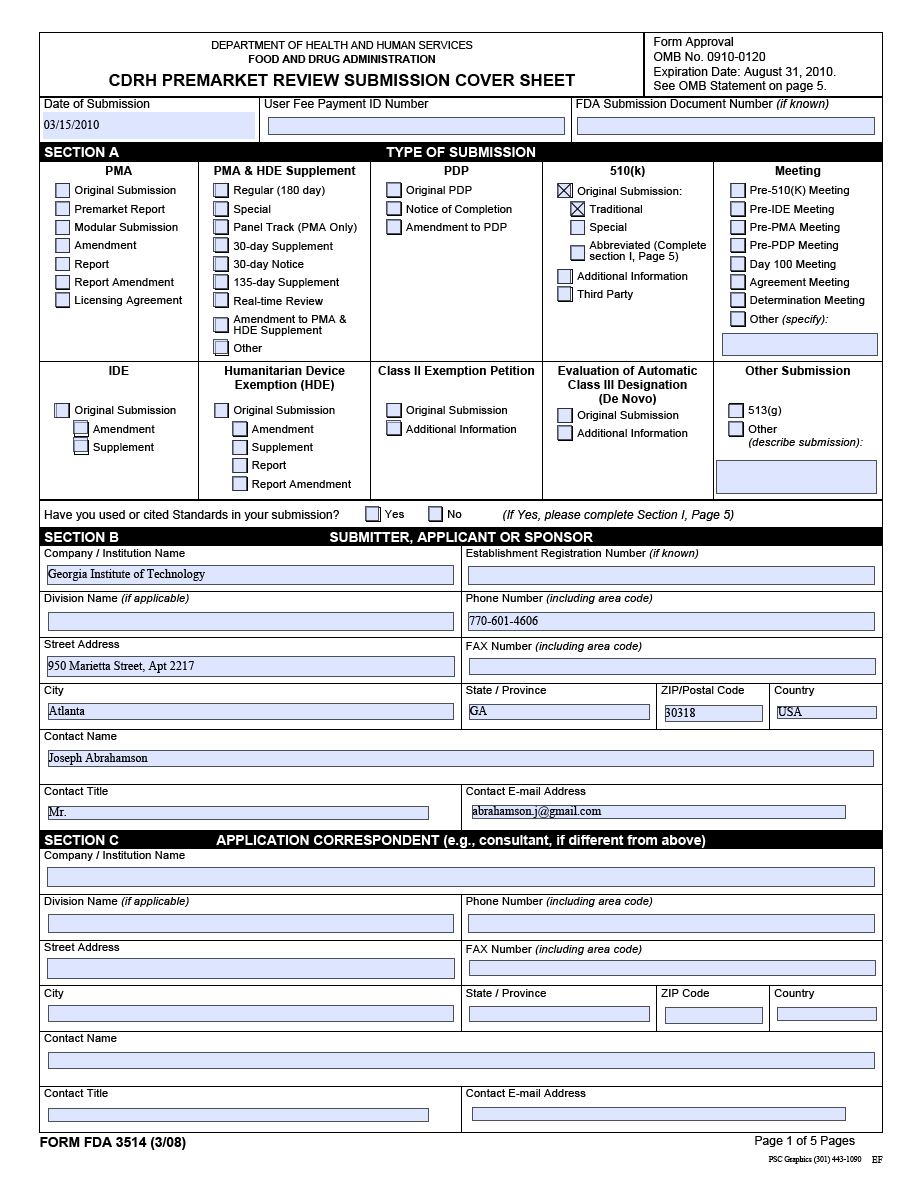
\includegraphics[width=1.2\linewidth]{pages/cdrh-pics/1}
  \label{fig:summary}
\end{figure}

\begin{figure}[H]
  \centering
  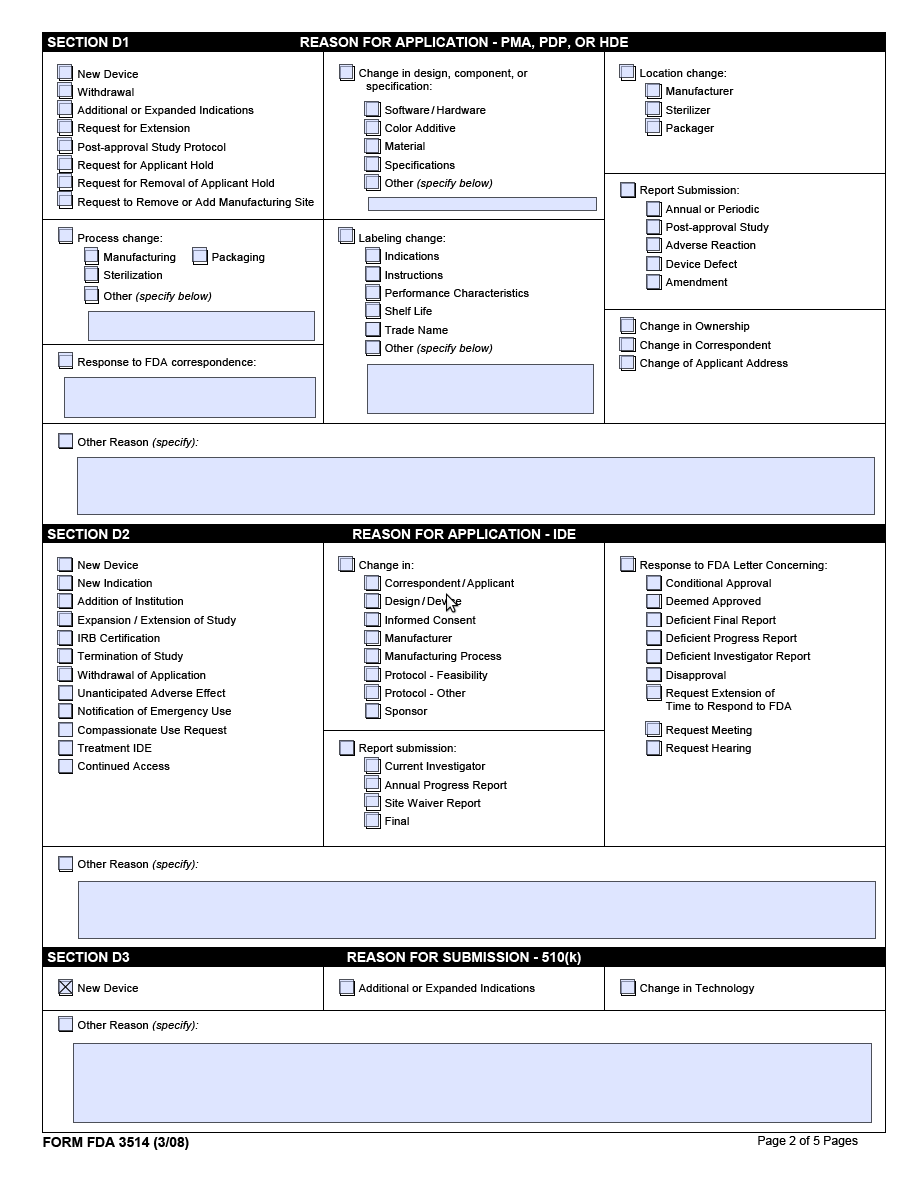
\includegraphics[width=1.2\linewidth]{pages/cdrh-pics/2}
  \label{fig:summary}
\end{figure}

\begin{figure}[H]
  \centering
  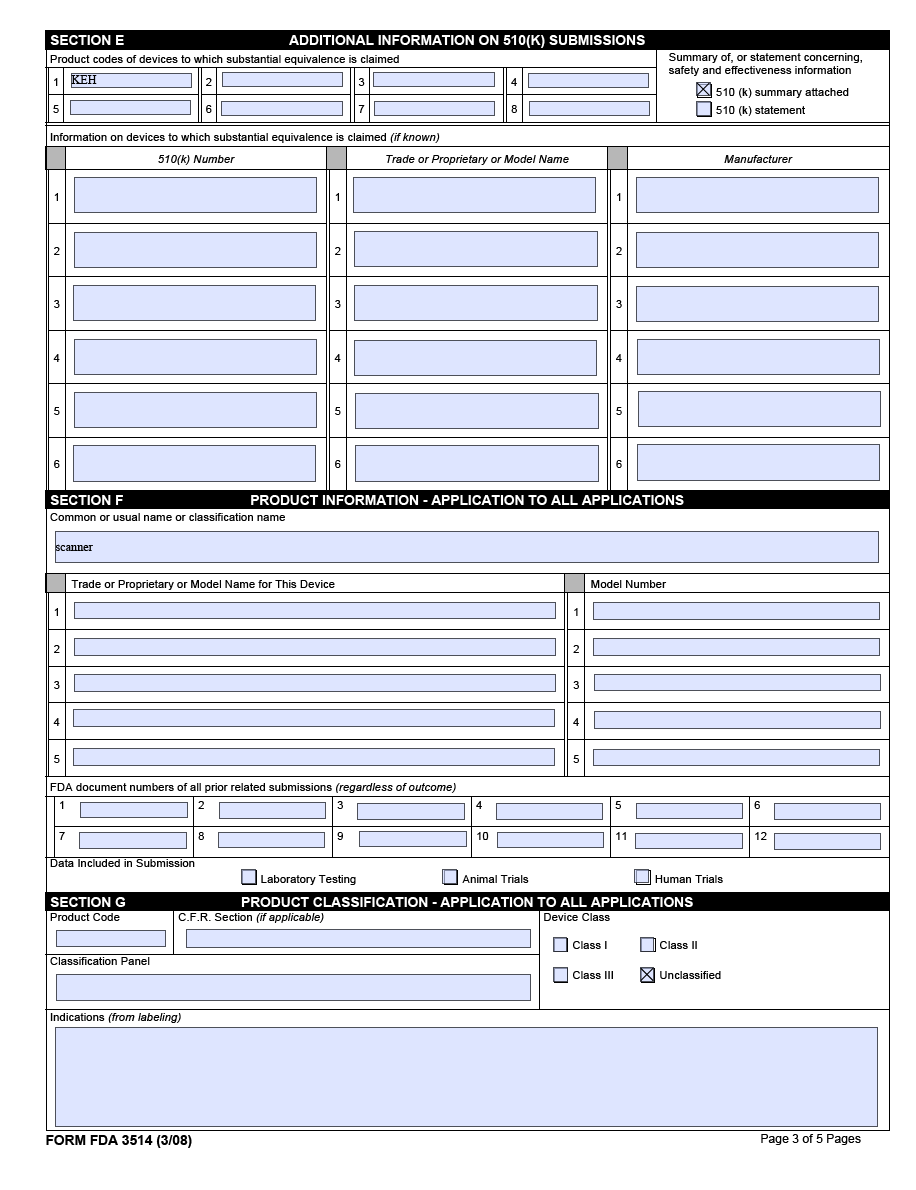
\includegraphics[width=1.2\linewidth]{pages/cdrh-pics/3}
  \label{fig:summary}
\end{figure}

\begin{figure}[H]
  \centering
  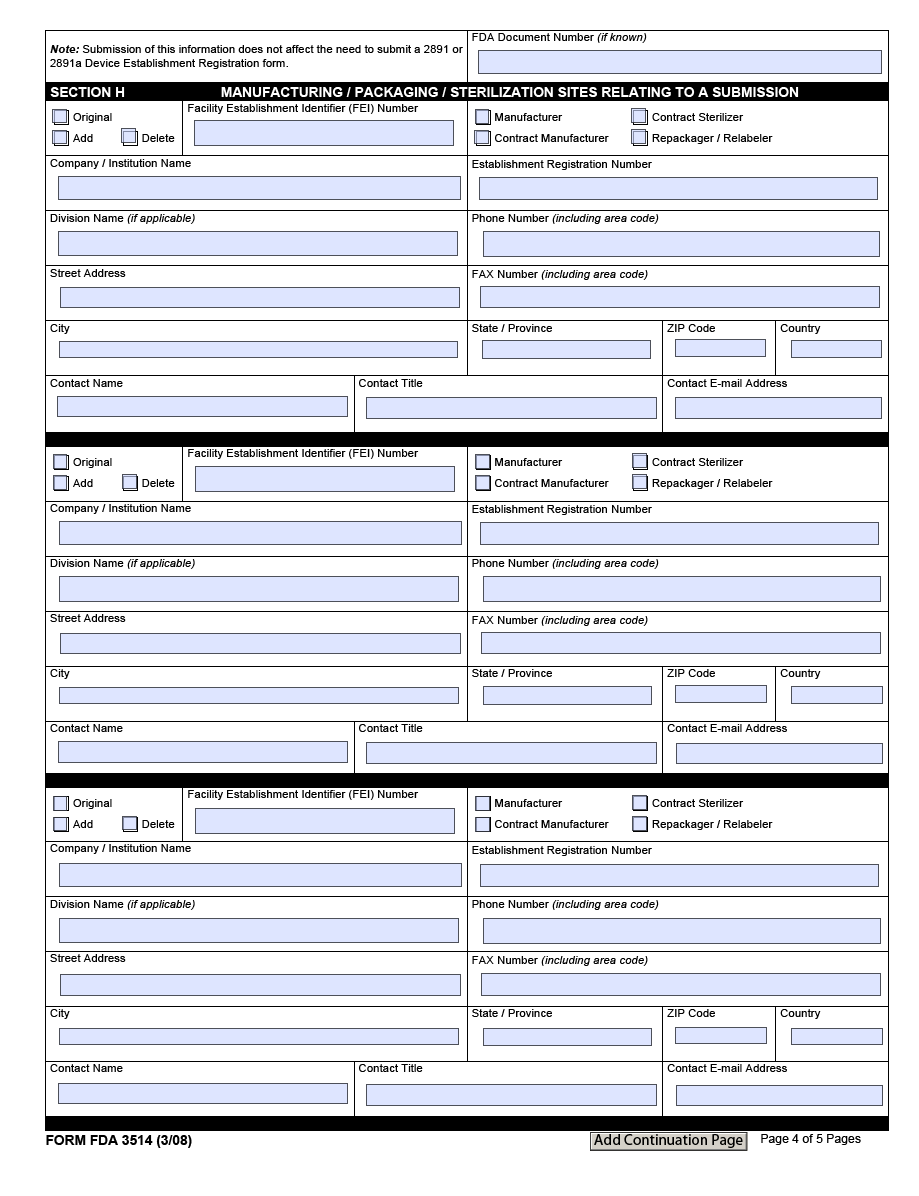
\includegraphics[width=1.2\linewidth]{pages/cdrh-pics/4}
  \label{fig:summary}
\end{figure}

\begin{figure}[H]
  \centering
  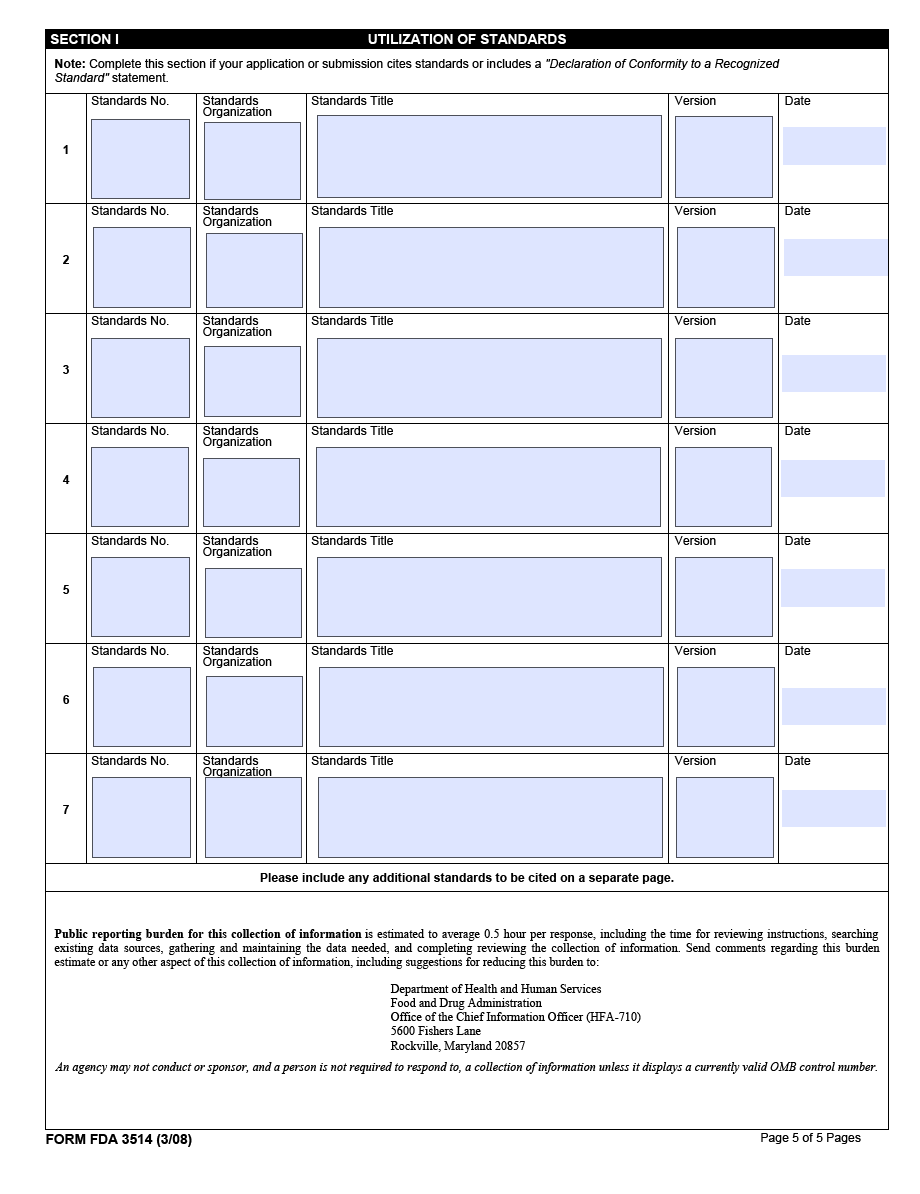
\includegraphics[width=1.2\linewidth]{pages/cdrh-pics/5}
  \label{fig:summary}
\end{figure}

%%% Local Variables: 
%%% mode: latex
%%% TeX-master: "../reg"
%%% End: 

\newpage
\addcontentsline{toc}{subsection}{510(k) Cover Letter}
\singlespacing

\begin{flushright}
  \huge{510(k) Submission --- Traditional}\\[.5in]
  
  \begin{minipage}{0.8\textwidth}
    \begin{flushright}
      \large \textbf{Scanner: eyeScan Mezzo} \\
      \textit{\today}
    \end{flushright}
  \end{minipage}
\end{flushright}

\begin{flushleft}
  Joseph Abrahamson\\
  $<$\textit{abrahamson.j@gatech.edu}$>$ \\
  Phone: 770 601 4606 \\[1em]
  
  \textit{Will register establishment following FDA clearance.}
\end{flushleft}
\vspace{4em}

\onehalfspacing

We seek FDA clearance to market our device, \textbf{eyeScan Mezzo}, a
Class II medical device used for medical scanning of three-dimensional
exterior eye shape. To our knowledge FDA has not classified this
device and, thus, no product code has been assigned or requested for
this device in the Classification Database. Substantially equivalent
devices belong to the General \& Plastic Surgery, Radiology, and
Pathology panels. This finished component is a novel device not
previously marketed with FDA clearance in the USA. We require 510(k)
clearance due to substantial equivalence with existent optical
coherence tomography devices (regulation no. \textbf{886.1570},
product code \textbf{OBO}), x-ray computed tomography devices
(regulation no. \textbf{892.1750}, product code \textbf{JAK}), and
microscopes, micrometers, and accessories (regulation
no. \textbf{864.3600}, product code \textbf{KEH}). Manufacturing
registration is currently unspecified. 

With regards to performance standards, this device contains electrical
components, and is subject to testing under IEC 60601-1-2 Part
I. Furthermore, the device contains a laser component, which under 21
CFR 1000 dictates that the device falls under RCHSA controls. RCHSA
controls indicate that the manufacture of the laser component of this
device is subject to standards 1002.10, 1002.13, and 1002.30, which
specifiy necessary reporting on the manufacturing of the laser
component. Lastly, while the device does contain a laser, it is exempt
from 21 CFR 1040.

%%% Local Variables: 
%%% mode: latex
%%% TeX-master: "../reg"
%%% End:


\newpage
\addcontentsline{toc}{subsection}{Indications for Use Statement}

\begin{center}
  \huge{Indications for Use Statement}\\[.5in]
\end{center}


\onehalfspacing

510(k) Number (if known): N/A \\
Device Name: eyeScan Mezzo \\
Indications for Use: 

%%% Local Variables: 
%%% mode: latex
%%% TeX-master: "../reg"
%%% End: 

\newpage
\addcontentsline{toc}{subsection}{510(k) Statement}
\singlespacing
\begin{center}
  \large{510(k) Statement}
\end{center}

\onehalfspacing


I certify that, in my capacity as product development scientist, I
will make available all information included in this premarket
notification on safety and effectiveness within 30 days of request by
any person if the device described in the premarket notification
submission is determined to be substantially equivalent. The
information I agree to make available will be a duplicate of the
premarket notification submission, including any adverse safety and
effectiveness information, but excluding all patient identifiers, and
trade secret and confidential commercial information, as defined in 21
CFR 20.61.

\begin{figure}[H]
  
\includegraphics[width=0.35\linewidth]{imgs/ja-sig}
\end{figure}

\noindent Joseph Abrahamson \\
\today


%%% Local Variables: 
%%% mode: latex
%%% TeX-master: "../reg"
%%% End: 

\newpage
\addcontentsline{toc}{subsection}{Truthful And Accurate Statement}
\singlespacing
\begin{center}
  \large{Truthful And Accurate Statement}
\end{center}

\onehalfspacing

I certify that, in my capacity as product development scientist, I
believe to the best of my knowledge, that all data and information
submitted in the premarket notification are truthful and accurate and
that no material fact has been omitted.

\begin{figure}[H]
  
\includegraphics[width=0.35\linewidth]{imgs/ja-sig}
\end{figure}

\noindent Joseph Abrahamson \\
\today

%%% Local Variables: 
%%% mode: latex
%%% TeX-master: "../reg"
%%% End: 

\newpage
\addcontentsline{toc}{subsection}{Class I Summary and Certification}
\singlespacing
\begin{center}
  \large{Class I Summary and Certification}
\end{center}

\onehalfspacing

I certify that, in my capacity as product development scientist that I
this device best claims substantial equivalence to a Class I device.

\begin{figure}[H]
  
\includegraphics[width=0.35\linewidth]{imgs/ja-sig}
\end{figure}

\noindent Joseph Abrahamson \\
\today

%%% Local Variables: 
%%% mode: latex
%%% TeX-master: "../reg"
%%% End: 
 % Certified SE to Class I instead of CIII
\newpage
\subsection{Financial Certification or Disclosure Statement}

I certify that, in my capacity as product development scientist that
no clinical studies were performed and thus no financial disclosure is
possible or required.

\begin{figure}[H]
  
\includegraphics[width=0.35\linewidth]{imgs/ja-sig}
\end{figure}

\noindent Joseph Abrahamson \\
\today

%%% Local Variables: 
%%% mode: latex
%%% TeX-master: "../reg"
%%% End: 

\newpage
\subsection{Declarations of Conformity and Summary Reports}

We chose to not rely on a recognized standard or guidance for any part
of the device design or testing. Instead, we have developed a set of
independent testing protocols. Device testing will be conducted using
this independently generated testing protocol and will meet specified
acceptence criteria before the device is marketed. 



% Real sections
\setcounter{subsection}{0}
\subsection{Executive Summary}
\subsection{Device Description}
\subsection{Substantial Equivalence Discussion}

\subsection{Proposed Labeling}

The device labeling will include three general categories: packaging,
marketing copy, and operation manuals. Due to the exception of section
502(f) as orchestrated by part 801.125, the operations manual will be
distributed electronically.

\subsubsection{Packaging}
The device is marketed at an operational research lab and therefore
does not require intensive package marketing. Instead an austere
recycled carboard box tied with twine is labeled simply with the
device name (eyeScan Mezzo) and appropriate device IDs.

\subsubsection{Operations Manual}
The operations manual will consist of an easily accessible electronic PDF document divided
into three subsections. The first will detail the process for making
the solution in which the eyeball is suspended; the second will
describe how to suspend the eyeball in solution; and the third will
consist of instructions for connecting the entire device to a
computer.

The suspension solution is polydimethylsiloxane (PDMS), to be made
using the Sylgard 184 Silicone Elastomer Kit included with the device. 1 gram of base solution
and 0.03 grams of curing agent are to be combined in an optical glass
tube at room temperature using a pipette. The resulting solution is to
be well mixed.

To suspend the eyeball in solution, the eyeball will be rinsed
using aqueous water. Inverted tweezers will be used to pick up the
eyeball by the optic nerve and gently suspend it in the center of the
tube containing polymer solution. The tube will then be capped tightly
and placed into the top slot of the scanning machine.

The device’s user interface will consist of two wires. One wire will
plug into a standard United States outlet of 120 V at 60 Hz and the
other will be a USB cable that plugs into a standard USB drive in a
computer. This will allow the device to transmit scanning data to a
computer for three-dimensional reconstruction. The device will also
have a power on/off switch at the back.

The Sylgard 184 Silicone Elastomer kit will include a brief operations
manual along with MSDS information in paper format.

\subsubsection{Marketing Copy}

\paragraph{Description}
The device, named eyeScan Mezzo, is a bench-sized digitizer able to  and intended to accurately measure and create digital meshes corresponding to the three-dimensional surface structure of dissected rat eyes. It is accurate to a 2 um resolution. EyeScan Mezzo is not intended for use in the diagnosis or treatment of diseases for live animals or humans. Device testing is conducted using developer generated testing protocol and will meet specified acceptance criteria before the device is marketed. Full testing of the device's EMC characteristics is performed according to IEC 60601-1-2 Part I.

\paragraph{Safety and Effectiveness Considerations}

EyeScan Mezzo is intended to be operated only by trained laboratory personnel in ophthalmological research settings only. It poses no known immediate health hazard to the operator. 

\paragraph{Contraindications, Warnings, Precautions}

PDMS is toxic to humans, and as such, contact with skin and organs should be avoided. If PDMS does come into contact with the skin, eyes, or body, one should immediately clean off PDMS from body part using a paper towel and rinse contaminated area under running water. Refer to the MSDS for further instruction.

Insertion of objects other than that indicated in the operations manual may damage the device.
If any foreign object enters the device, the operator should turn off the device and cut off the power supply to the device immediately. The operator should then remove the protection casing of the device, remove the foreign object, and reinstall the protection casing. If the device is damaged to the point of malfunction, the operator should contact the manufacturer for repairs. 

A liquid spill inside the machine may damage electronic components and pose an electrical hazard.
If a liquid spill occurs, the operator should turn off the device and cut off the power supply to the device immediately. The operator should then send in a request to the manufacturer to replace damaged parts.

Proper laboratory attire such as latex gloves, laboratory coats, and goggles should be worn before operating the device. 

Injury may result if the device is operated by untrained personnel. 


%%% Local Variables: 
%%% mode: latex
%%% TeX-master: "../reg"
%%% End: 

\newpage
\subsection{Sterilization and Shelf Life}

This device is not sold as sterile. During operation, sterility
does not impact the safety of effectiveness of the device.

\newpage
\subsection{Biocompatibility}

This device contains no components which come into direct or indirect
contact with patients. The device is intended for use in research
settings, not clinical settings.

Furthermore, we claim substantial equivalence with microscopes and
accessories (regulation number: 864.3600, product code:
KEH). Microscopes and accessories are identified as optical
instruments used to enlarge images of specimens, preperations, and
cultures for medical purposes. Our device thus makes use of identical
materials used in devices claimed to be substantially equivalent, as
it is intended for use with dissected eyeballs. 


\subsection{Software}

\subsection{Electromagnetic Compatibility and Electrical Safety}

Our device does contain a number of sensitive electronic
devices. Electrical failure of the device cannot result in safety
hazards as under electrical interference the device will simply fail
to deliver results. Additionally, the components of the device are
hardened to electrical shock and resonance. Full testing of the
device's EMC characteristics will be performed according to IEC
60601-1-2 Part I.

There is no patient contact with electrical components of the device
as the device is intended to be used exclusively with dissected
eyeballs in research settings.


%%% Local Variables: 
%%% mode: latex
%%% TeX-master: "../reg"
%%% End: 


%\subsection{Performance Testing --- Lab, Animal, Clinical}
% Not required

\section{Discussion}
\label{sec:discussion}

\section{Conclusion}
\label{sec:conclusion}


\newpage
\addcontentsline{toc}{section}{References}
\bibliographystyle{unsrt}
\bibliography{../tex/bibl}

\end{document}
%%% Local Variables: 
%%% mode: latex
%%% TeX-master: t
%%% End: 
